  \let\negmedspace\undefined
\let\negthickspace\undefined
\documentclass[journal]{IEEEtran}
\usepackage[a5paper, margin=10mm, onecolumn]{geometry}
\usepackage{lmodern} % Ensure lmodern is loaded for pdflatex
\usepackage{tfrupee} % Include tfrupee package

\setlength{\headheight}{1cm} % Set the height of the header box
\setlength{\headsep}{0mm}     % Set the distance between the header box and the top of the text

\usepackage{gvv-book}
\usepackage{gvv}
\usepackage{cite}
\usepackage{amsmath,amssymb,amsfonts,amsthm}
\usepackage{algorithmic}
\usepackage{graphicx}
\usepackage{textcomp}
\usepackage{xcolor}
\usepackage{txfonts}
\usepackage{listings}
\usepackage{enumitem}
\usepackage{mathtools}
\usepackage{gensymb}
\usepackage{comment}
\usepackage[breaklinks=true]{hyperref}
\usepackage{tkz-euclide} 
\usepackage{listings}                                      
\def\inputGnumericTable{}                                 
\usepackage[latin1]{inputenc}                                
\usepackage{color}                                            
\usepackage{array}                                            
\usepackage{longtable}
\usepackage{multicol}
\usepackage{calc}                                             
\usepackage{multirow}                                         
\usepackage{hhline}                                           
\usepackage{ifthen}                                           
\usepackage{lscape}
\begin{document}
	
	\bibliographystyle{IEEEtran}
	\vspace{3cm}
	
	\title{11.16.3.3.5}
	\author{EE24BTECH11059 - Y Siddhanth}
	% \maketitle
	% \newpage
	% \bigskip
	{\let\newpage\relax\maketitle}
	
	\renewcommand{\thefigure}{\theenumi}
	\renewcommand{\thetable}{\theenumi}
	\setlength{\intextsep}{10pt} % Space between text and floats
	
	
	\numberwithin{equation}{enumi}
	\numberwithin{figure}{enumi}
	\renewcommand{\thetable}{\theenumi}
	
	
\textbf{Question}:\\
A die is thrown, find the probability of a number less than 6 to appear is?
\\
\textbf{Solution: }\\
The sample space (\( \Omega \)) for rolling a die is:
\begin{align}
\Omega = \{1, 2, 3, 4, 5, 6\}
\end{align}
Each outcome is equally likely.
Let the random variable \( X \) represent the number rolled on the die.\\
Probability Mass Function (PMF): \\
The PMF for a fair die is:
\begin{align}
P(X = x) =
\begin{cases}
	\frac{1}{n}, & k \in \{1, 2,\dots ,n\} \\
	0, & \text{otherwise}
\end{cases}
\end{align}
Cumulative Distribution Function (CDF): \\
The CDF for the die roll is:
\begin{align}
	F_X(k) = P(X \leq k) =
	\begin{cases}
		0, & k < 1 \\
		\frac{k}{n}, & 1 \leq k < n\\
		1, & k \geq n
	\end{cases} \label{cdf}
\end{align}
Where n is 6. \\ 
$\therefore$ The probability of getting a number less than 6 is as below, from \eqref{cdf}
\begin{align}
	P\brak{X < 6} &= F_X(5) \\  &= \frac{5}{6}
\end{align} 
Probability simulation: \\ 
We will use the hardware random number generator of an ESP32 to simulate true randomness. 
I have referred the esp32-technical-reference-manual, for the proper usage of it's random number generator. These true random numbers are generated based on the thermal noise in the system
and the asynchronous clock mismatch.
	\begin{figure}[h!]
	\centering
	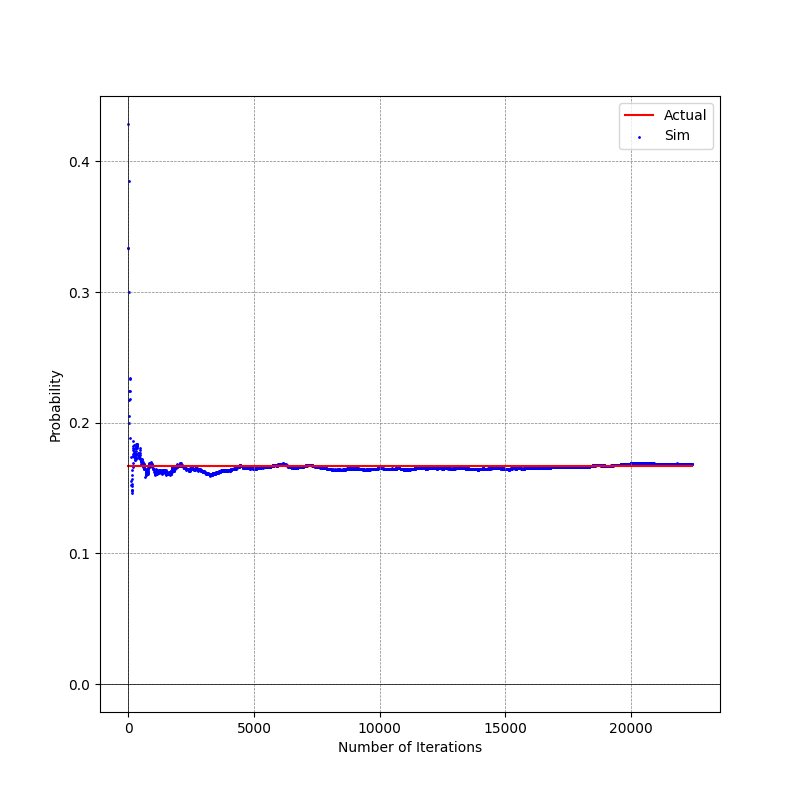
\includegraphics[width=\columnwidth]{figs/sim.png}
	\caption{Simulation using ESP32}
\end{figure}
	
		\begin{figure}[h!]
		\centering
		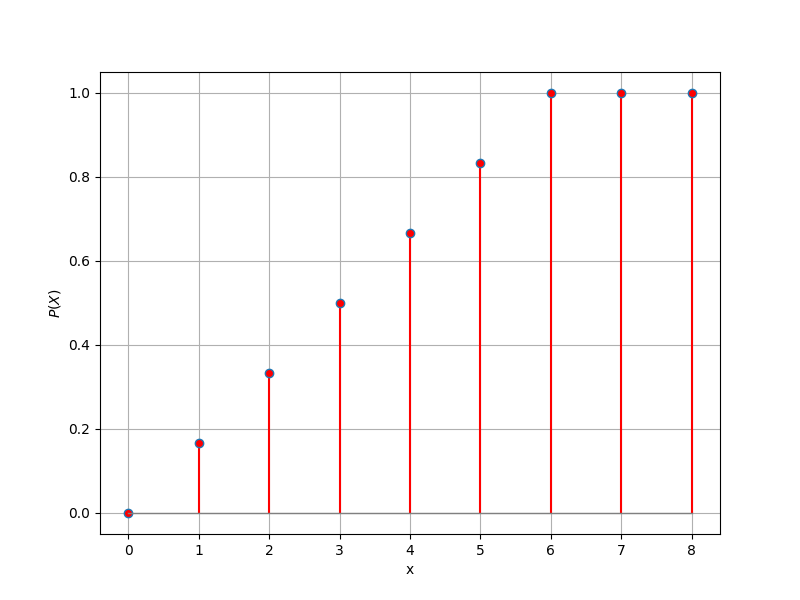
\includegraphics[width=\columnwidth]{figs/cdf.png}
		\caption{Cumulative Distribution Function}
	\end{figure}
\end{document}  